\section{Unclaimed Letters at the Cape of Good Hope Post Offices}



\ph[width = .90\textwidth]{../cape-of-good-hope/Advertized-and-Unclaimed/Advertized-and-Unclaimed-postmark.jpg}{
Postcard addressed to Durban South Africa 
and re-directed to 'Post-Restante' Cape Town, bearing 'Post-Restante' 
single circle postmark, Return Letter Office dated Apr 06 when it was also 
stamped 'ADVERTIZED and UNCLAIMED'. 
(After some four months or so lying by the 'POST RESTANTE' section.}


	 


In the early days of the Cape of Good Hope letters were often addressed to private individuals marked 'to be called for'.

After a certain time has lapsed these 'UNCLAIMED' letters were postmarked with one of 
the the Return Letter postmarks (Goldblatt RLO 16 to RL 18).

As these undelivered letters accumulated the postoffice periodically published lists in the 'Cape Government Gazette'. If after a certain period they were still not claimed they were stamped with one of the postmarks illustrated (Goldblatt RL0 19 to RLO 23) and then kept for a few more months.

\begin{figure}[htbp]

\includegraphics[width=0.95\textwidth]{../cape-of-good-hope/Advertized-and-Unclaimed/Unclaimed-postmarks.jpg}
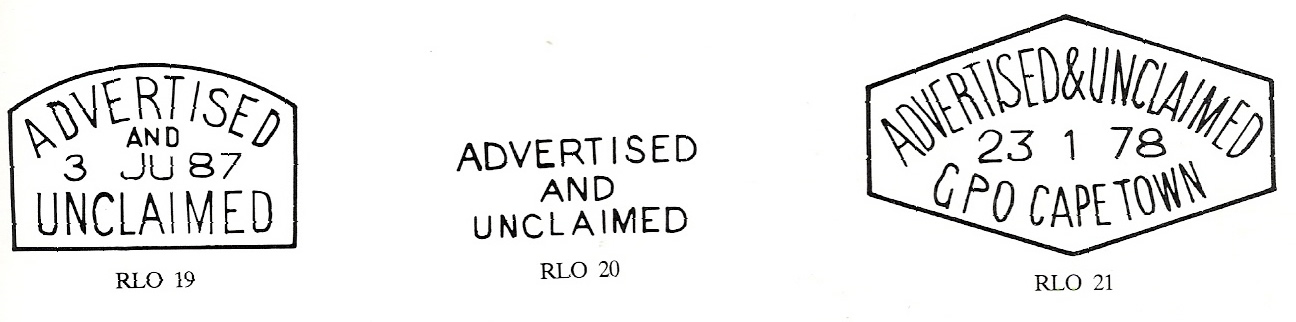
\includegraphics[width=0.95\textwidth]{../cape-of-good-hope/Advertized-and-Unclaimed/Advertized-and-Unclaimed-Postmarks.jpg}

\includegraphics[width=0.95\textwidth]{../cape-of-good-hope/Advertized-and-Unclaimed/Advertized-and-Unclaimed-Postmarks-2.jpg}
\caption{Advertized and unclaimed marks of the Cape of Good Hope (from Goldblatt).}
\end{figure}

Eventually these letters were opened their content examined and if 
they contained valuables such as coins or notes their content 
was recorded before they were destroyed by the Cape Postal authorities.

Some of these letters survived and one of them is illustrated above.
Advertized and Unclaimed Cape Postmarks. How, they survived? 
It is not known but possibly some were eventually collected 
before they were destroyed and others might have found their way 
into the philatelic market the same way proofs and essays do.


 
	 
  	

 


 

 

               